\RequirePackage{fix-cm}
\documentclass{article}
\usepackage{graphicx}
\usepackage{background}
\usepackage{tikz}
\usepackage{float}
\usepackage{eso-pic}
\usepackage{hyperref}


% Imposta il background per la prima pagina
\backgroundsetup{
    scale=1,
    color=black,
    opacity=1,
    angle=0,
    contents={
        \begin{tikzpicture}[overlay, remember picture]
            \node[inner sep=0pt, anchor=center] at (current page.center) {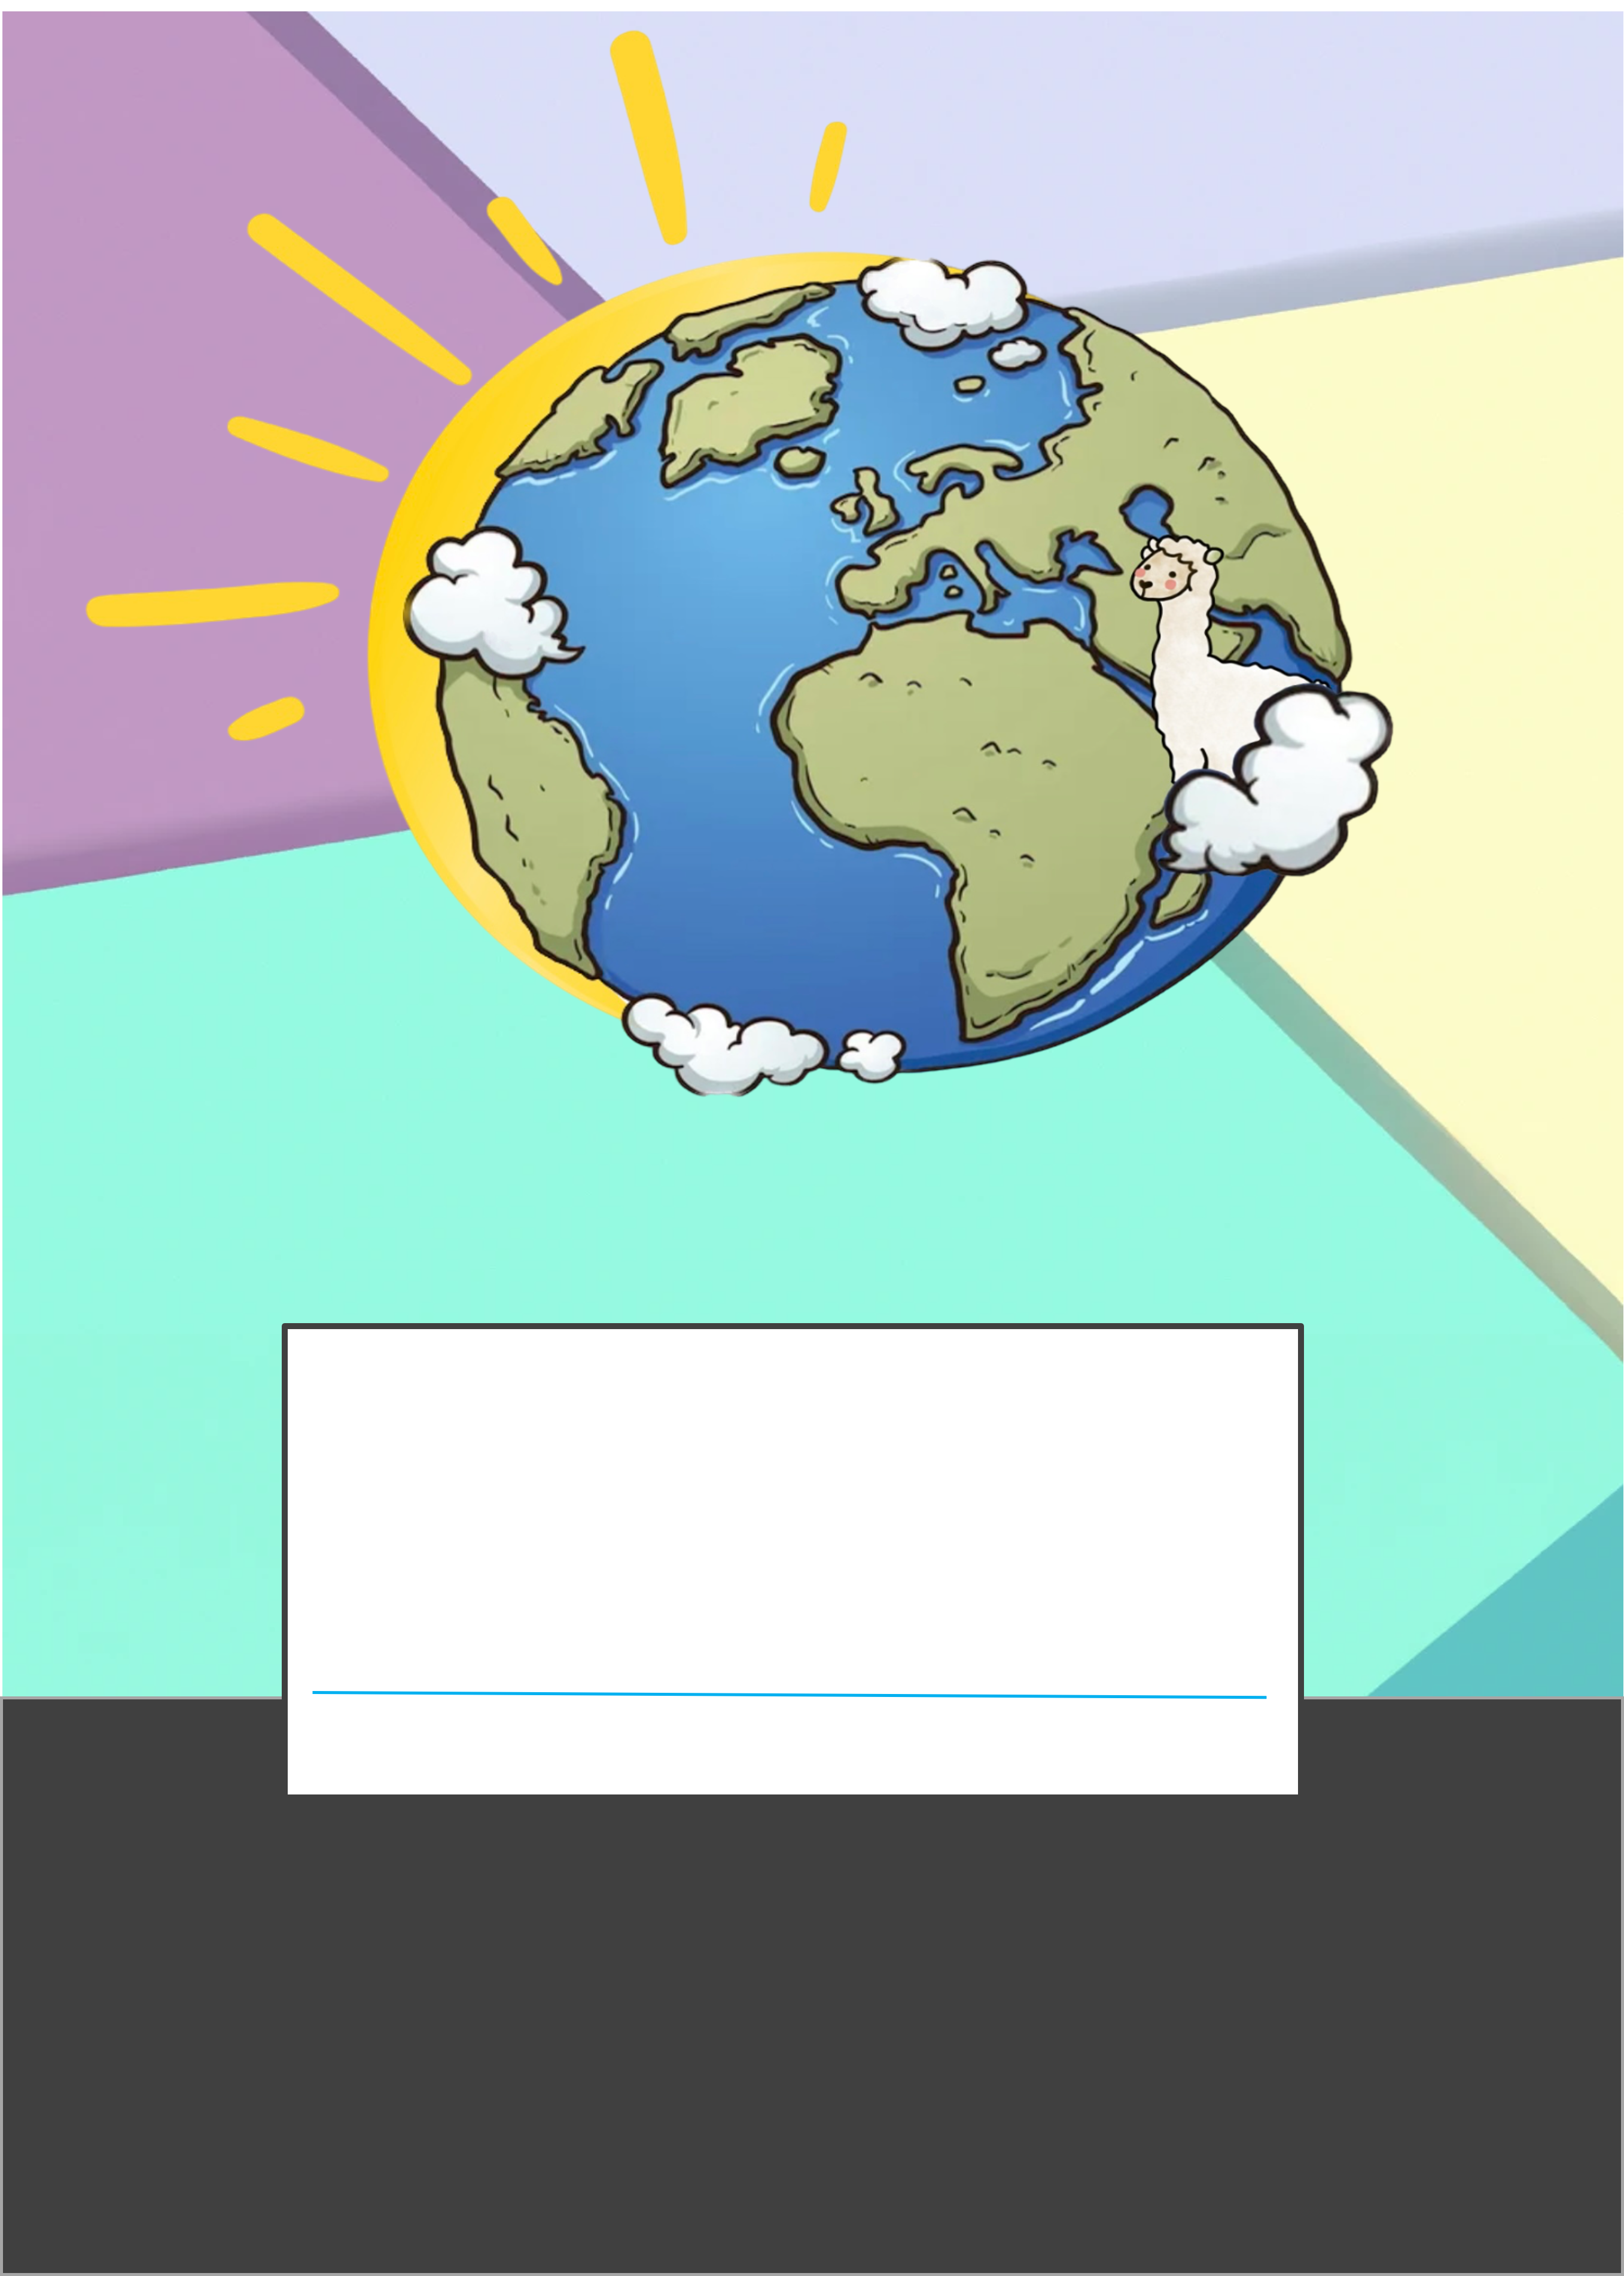
\includegraphics[width=\paperwidth,height=\paperheight,keepaspectratio]{../../img/firstpage_background.png}};
            \node[text=cyan, font=\fontsize{35}{50}\selectfont\bfseries] at ([xshift=-0.2cm,yshift=-4.5cm]current page.center) {Climate Monitoring};
            \node[text=cyan, font=\large] at ([xshift=-0.4cm,yshift=-7.5cm]current page.center) {\textit{Manuale Tecnico}};
            \node[text=white, font=\large] at ([xshift=-8.5cm,yshift=-9cm]current page.center) {Autori:};
            \node[text=white, font=\large] at ([xshift=-6.85cm,yshift=-10.5cm]current page.center) {Andrea Tettamanti 745387};
            \node[text=white, font=\large] at ([xshift=-7.28cm,yshift=-11.5cm]current page.center) {Luca Mascetti 752951};
            \node[text=white, font=\large] at ([xshift = 8cm, yshift = -9cm]current page.center) {Versione: 1.1};
            \node[text=white, font=\large] at ([xshift = 8cm, yshift = -10cm]current page.center) {Data: 07-02-2024};
        \end{tikzpicture}    }
}



\begin{document}



%frontespizio
\begin{titlepage}
    \null
\end{titlepage}

% Sovrapponi l'immagine al numero di pagina
\AddToShipoutPictureBG{
    \begin{tikzpicture}[overlay, remember picture]
        \node[inner sep=0pt, anchor=south] at ([xshift=-0.15cm,yshift=2.7cm]current page.south) {
\includegraphics[width=1.5cm,height=1.5cm]{../../img/number page.png}};
    \end{tikzpicture}
}

\clearpage
\NoBgThispage
\tableofcontents
\listoffigures
\clearpage


\NoBgThispage
\section{Introduzione}
Benvenuti nell'applicazione \emph{Climate Monitoring}, software progettato per fornire accesso ai dati climatici 
provenienti dai centri di monitoraggio in tutta Italia. Questa applicazione è stata sviluppata con l'obiettivo di 
mettere a disposizione degli operatori ambientali e dei cittadini comuni dati accurati e rilevanti relativi alle 
condizioni climatiche della propria zona di interesse.

\NoBgThispage
\section{Struttura Generale dell'Applicazione}
L’applicazione è stata sviluppata seguendo l’architettura \texttt{MVC (Model-View-Controller)}, dove le parti View e Controller sono inglobati nella User Interface (UI).
Di conseguenza il codice sorgente del package \texttt{src} è suddiviso in due Macro-package: \texttt{Models} in cui sono presenti tutte le classi che gestiscono i dati,
mentre nel package \texttt{GUI} sono presenti le classi che gestiscono la UI e l’interazione tra i comandi fatti dall’utente e lo storage dei dati.
È presente anche un package, \texttt{utils}, che contiene classi di utilità usate nella maggior parte delle altre classi.


\begin{figure}[H]
    \centering
    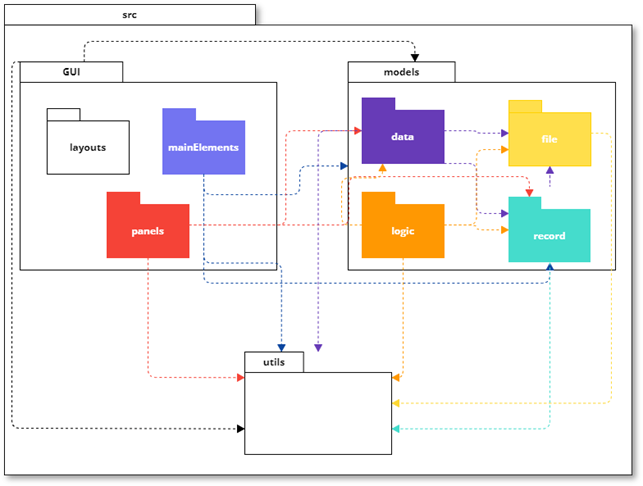
\includegraphics[width=0.7\textwidth]{../../img/package_structure.png}
    \caption{Struttura dei package dell'applicazione.}
\end{figure}
\section{Strutture Dati e scelte Algoritmiche}
I dati vengono salvati in modo definitivo in un file \texttt{.csv}. Quando si apre l'applicazione, i dati contenuti nei file vengono letti e caricati in delle mappe strutturate
come relazioni in un database (chiave primaria + tupla), da cui poi estrarre i dati quando richiessto.\\
Abbiamo scelto di utilizzare le \texttt{HashMap} per diversi motivi. In primo luogo, l'uso di una \texttt{HashMap} in memoria offre un accesso rapido ed efficinete ai dati. 
Una volta che i dati sono stati letti dai file, vengono memorizzati in memoria sottoforma di \texttt{HashMap}, consentendo operazioni di accesso rapido con complessità $O(1)$.\\ 
Lavorare direttamente sui file avrebbe richiesto operazioni di lettura e scrittura più frequenti, coinvolgendo l'I/O del disco, che è generalmente più lento rispetto all'I/O in memoria.
Memorizzare i dati in una \texttt{HashMap} consente di evitare la necessità di aprire e chiudere frequentemente i file durante le operazioni.\\
Inoltre, le \texttt{HashMap} forniscono una struttura dati efficiente per la gestione di associazioi chiave-valore. Questo è particolarmente utile nel nostro caso, dova abbiamo bisogno
di eseguire operazioni di ricerca, inserimento e aggiornamento dei dati in modo veloce ed efficiente.\\
Alcune della altre strutture dati potrebbero essere meno adatte alle esigenze specifiche del progetto. Ad esempio, le liste potrebbero risultare inefficaci per le operazioni di ricerca 
rapida, mentre altre strutture dati complesse, come alberi, grafi o liste di liste, potrebbero aggiungere una complessità non necessaria alla nostra implementazione.\\
\\
Ora verranno descritte le sclete algoritmiche e le loro complessità della parte \texttt{Model} del progetto, in quanto è la sezione che si occupa della gestione dei dati.\\
\\
\textbf{DataStorage}
\begin{enumerate}
    \item Creazione delle Mappe:
    \begin{itemize}
        \item Inizializzazione nel costruttore tramite i metodi \texttt{createCityMap(), createOperatorMap(), createCenterMap(), e createWeatherMap()}.
        \item Ogni metodo legge i dati dal file corrispondente utilizzando \texttt{FileHandler} e costruisce oggetti (es. \texttt{RecordCity, RecordOperator}, ecc.)
        per l'inserimento nella mappa corrispondente.
        \item Complessità: $O(n)$, dove $n$ è il numero di record nel file. 
    \end{itemize}
    \item Operazioni di Ricerca:
    \begin{itemize}
        \item Fornisce metodi (es. \texttt{getCityByID, getOperatorByID, getCenterByID, getWeatherByID}) per recuperare oggetti specifici dalla mappa basandosi sull'ID.
        \item Complessità: $O(1)$, per accesso in una \texttt{HashMap}.
    \end{itemize}
\end{enumerate}

\textbf{DataQuery}
\begin{enumerate}
    \item Metodi di Recupero per Singole Entità:
    \begin{itemize}
        \item Utilizzando il metodo privato\texttt{filterData} per filtrare i dati basandosi su condizioni specifiche.
        \item Complessità: $O(n)$, dove $n$ è il numero di elementi nella collezione.
    \end{itemize}
    \item Metodi di Filtraggio Interni:
    \begin{itemize}
        \item Verificano se un elemento soddisfa una condizione specifica.
        \item Complessità: $O(1)$, ma totale dipende dal numero di condizioni.
    \end{itemize}
    \item Generazione di Epsilon:
    \begin{itemize}
        \item Il metodo \texttt{generateEpsilon} calcola un valore di $\epsilon$ basato sul numero di posizioni deciamli di un dato valore.
        \item Complessità: $O(n)$, dove $n$ è il numero di posizioni decimali.
    \end{itemize}
    \item Caloclo delle Posizioni Decimali:
    \begin{itemize}
        \item Il metodo \texttt{computeDecimalPositions} calcola il numero di posizioni decimali di un valore \texttt{double}.
        \item Complessità: $O(n)$, dove $n$ è la lunghezza della stringa rappresentante il valore.
    \end{itemize}
\end{enumerate}

\textbf{DataHandler}
\begin{enumerate}
    \item Generazione della Chiave Primaria:
    \begin{itemize}
        \item Il metodo \texttt{generatePrimaryKey} cerca iterativamente la chiave $k$ più alta della mappa attuale e genera una nuova chiave $k' = {k+1}$.
        \item Complessità: $O(n)$, dove $n$ è il numero di elementi nella mappa.
    \end{itemize}
    \item Aggiunta di nuovi Record Operatore, Centro e dati Meteorologici:
    \begin{itemize}
        \item Il metodo \texttt{addNewRecord} genera un nuovo record, verifica se ci sono duplicati, aggiunge il record nella relativa mappa e scrive i dati nel file corrispondente.
        \item Complessità: $O(n)$, dove $n$ è il numero di record già presenti.
    \end{itemize}
    Aggiornamento di Record:
    \begin{itemize}
        \item Il metodo \texttt{updateRecord} ricerca il record nel file, lo aggiorna e riscrive il file con il nuovo record.
        \item Complessità: $O(n)$, dove $n$ è il numero totale di righe nel file.
    \end{itemize}
\end{enumerate}

\textbf{LogicCenter}
\begin{enumerate}
    \item Inizializzazione di un nuovo Centro di Monitoraggio:
    \begin{itemize}
        \item Algorimto con controlli su autenticazione, associazione dell'utene a un centro esistente, validità parametri del nuovo centro e verifica validità ID città.
        \item Aggiorna i dati dell'operatore quando viene associato al nuovo centro.
        \item Complessità: $O(n)$, dove $n$ è il numero di città associate al centro.
    \end{itemize}
    \item Aggiunta di dati meteorologici a un centro:
    \begin{itemize}
        \item Controlli sull'autenticazione dell'utente, associazione a un centro, validità della data e dei dati meteorologici.
        \item Aggiorna i dati della mappa e del file corrispondente aggiungendo un nuovo record di dati meteorologici.
        \item Complessità: $O(n)$, dove $n$ è il numero di righe di dati meteorologici fornite.
    \end{itemize}
\end{enumerate}

\textbf{LogicCity}
\begin{enumerate}
    \item Costruttore \texttt{WeatherTableData}:
    \begin{itemize}
        \item Construttore con array di record di dati meteorologici e chiamata a \texttt{processCategory} per ogni categoria presente nei record.
        \item Complessità:$O(n*m)$, dove $n$ è la lunghezza dell'array e $m$ è il numero di categorie.
    \end{itemize}
    \item Metodo \texttt{processCategory}:
    \begin{itemize}
        \item Aggiorna i punteggi, i conteggi dei record e i commenti per la categoria data.
        \item Complessità: $O(1)$ per ogni chiamata.
    \end{itemize}
    \item Metodo \texttt{getCategoryAvgScore}:
    \begin{itemize}
        \item Calcola la media dei punteggi per una categoria data.
        \item Complessità: $O(1)$.
    \end{itemize}
    \item Metodo \texttt{getCategoryRecordCount}:
    \begin{itemize}
        \item Ottiene il conteggio dei record per una categoria data.
        \item Complessità: $O(1)$.
    \end{itemize}
    \item Metodo \texttt{getCategoryComments}:
    \begin{itemize}
        \item Ottine la lista di commenti per una categoria data.
        \item Complessità: $O(1)$.
    \end{itemize}
\end{enumerate}

\textbf{LogicOperator}
\begin{enumerate}
    \item Algoritmo di Login \texttt{performLogin}:
    \begin{itemize}
        \item Verifica se i campi per il login non sono vuoti, esegue il \texttt{logout} se un operatore è già loggato, costruiisce la lista di condizioni per la query da effettuare
        e la esegue per ottenere l'operatore corrispondente alle credenziali fornite.
        \item Complessità: $O(n)$, dove $n$ è il numero di operatori registrati.
    \end{itemize}
    \item Algoritmo di Registrazione \texttt{performRegistration}:
    \begin{itemize}
        \item Controlli di validità su nome, cognome, codice fiscale, e-mail, username e password.
        \item Aggiunge un nuovo record alla mappa corrispondente.
        \item Complessità: $O(1)$, in quanto le operazioni sono indipendenti dal numero di operatori registrati.
    \end{itemize}
    \item Algoritmo di Associazione a un Centro \texttt{associateCenter}:
    \begin{itemize}
        \item Verifica se l'operatore è loggato ed aggiorna l'operatore corrente con l'ID del centro specificato.
        \item Complessità: $O(1)$, in quanto coinvolge solo operazioni di aggiornamento nella mappa.
    \end{itemize}
    \item Algoritmo di Validazione dei Dati:
    \begin{itemize}
        \item Controlli di validità sui dati froniti.
        \item Complessità: $O(n)$, dove $n$ è il numero di campi da controllare.
    \end{itemize}
    \item Algoritmo di Hashing della Password \texttt{hashPassword}:
    \begin{itemize}
        \item E' utilizzato l'algoritmo \texttt{SHA-256} combinato con la concatenazione di username e password.
        \item Complessità: $O(n)$, dove $n$ è la lunghezza dell'input in bit.
    \end{itemize}
\end{enumerate}

\textbf{RecordCity, RecordOperator, RecordCenter, RecordWeather}
\begin{enumerate}
    \item Costruttore del Record:
    \begin{itemize}
        \item Assegna i valori forniti ai campi del record.
        \item Complessità: $O(1)$.
    \end{itemize}
    \item Metodo \texttt{toString}: 
    \begin{itemize}
        \item Restituisce una rappresentazione testuale del record.
        \item Complessità: $O(n)$, dove $n$ è la lunghezza dell'array dei campi.
    \end{itemize}
\end{enumerate}

\textbf{CurrentOperator}
\begin{enumerate}
    \item Pattern Singleton:
    \begin{itemize}
        \item Implementato con una variabile statica privata \texttt{instance} e costruttore privato.
        \item \texttt{getInstance()} restituisce l'instanza unica di \texttt{CurrentOperator}.
        \item Complessità: $O(1)$, coinvolge solo operazioni di controlloe e allocazione di memoria.
    \end{itemize}
    \item Pattern Observer:
    \begin{itemize}
        \item Metodi \texttt{addCurrentUserChangeListener} e \texttt{removeCurrentUserChangeListener} gestiscono l'aggiunte e la rimozione di listener per i cambiamenti di utente.
        $O(1)$ per entrambi.
        \item Metodo \texttt{notifyCurrentUserChange} notifica tutti i listener registrati di un cambio di utente.
        $O(n)$, dove $n$ è il numero di listener registrati.
        \item Metodo \texttt{setCurrentOperator} imposta l'operatore corrente e notidica i listener solo se l'operatore è diverso da quello corrente.
        $O(n)$, per la chiamata a \texttt{notifyCurrentUserChange}.
    \end{itemize}
\end{enumerate}
\section{Pattern utilizzati}

All’interno della classe \texttt{CurrentOperatore.java} sono stati utilizzati due pattern specifici: il \textbf{Singleton} e \textbf{l’Observer}.\\
Il pattern Singleton è utilizzato per garantire che ci sia una sola istanza della classe \texttt{CurrentOperator} nell'applicazione. La classe ha un costruttore privato e un campo statico \texttt{instance}
che rappresenta l'istanza unica della classe. Il metodo \texttt{getInstance()} restituisce l'istanza esistente se è già stata creata o ne crea una nuova se non esiste ancora.
\begin{figure}[H]
    \centering
    \includegraphics[width=1\textwidth]{../../img/Singleton.png}
    \caption{Costruttore della classe CurrentOperator}
    \label{fig:Singleton}
    
\end{figure}

Questo pattern è stato implementato seguendo questo schema:
\begin{figure}[H]
    \centering
    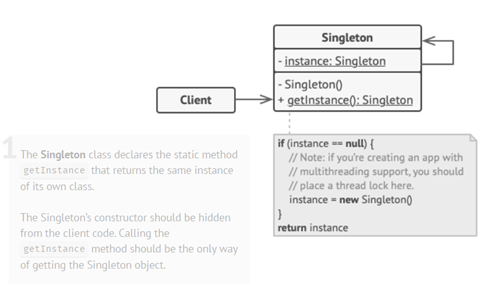
\includegraphics[width=1\textwidth]{../../img/schema_singleton.png}
    \caption{Schema del pattern Singleton}
    \label{fig:SingletonPattern}
    
\end{figure}

Il pattern Observer è utilizzato per notificare altri oggetti quando l'utente corrente cambia. La classe\texttt{CurrentOperator} definisce un'interfaccia \texttt{CurrentUserChangeListener}
che deve essere implementata da tutte le classi interessate ai cambiamenti dell'utente corrente.
\begin{figure}[H]
    \centering
    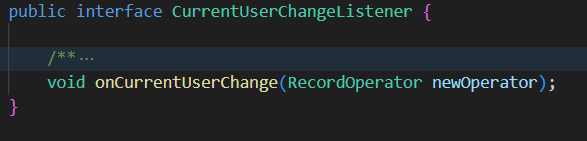
\includegraphics[width=1\textwidth]{../../img/currentUserChangeListener.png}
    \caption{Interfaccia CurrentUserChangeListener}
    \label{fig:Observer 1}
\end{figure}
La classe contiene metodi per aggiungere (\texttt{addCurrentUserChangeListener}) e rimuovere (\texttt{removeCurrentUserChangeListener}) listener interessati ai cambiamenti dell'utente corrente.
Quando l'utente corrente cambia, il metodo \texttt{notifyCurrentUserChange} viene chiamato per notificare tutti i listener registrati.
\begin{figure}[H]
    \centering
    \includegraphics[width=1\textwidth]{../../img/notifyCurrentUserChange.png}
    \caption{Metodo notifyCurrentUserChange}
    \label{fig:Observer 2}
\end{figure}
In questo modo, altre parti dell'applicazione possono essere avvisate quando l'utente corrente cambia, consentendo una gestione flessibile degli eventi correlati all'utente.

Questo pattern è stato implementato seguendo questo schema:
\begin{figure}[H]
    \centering
    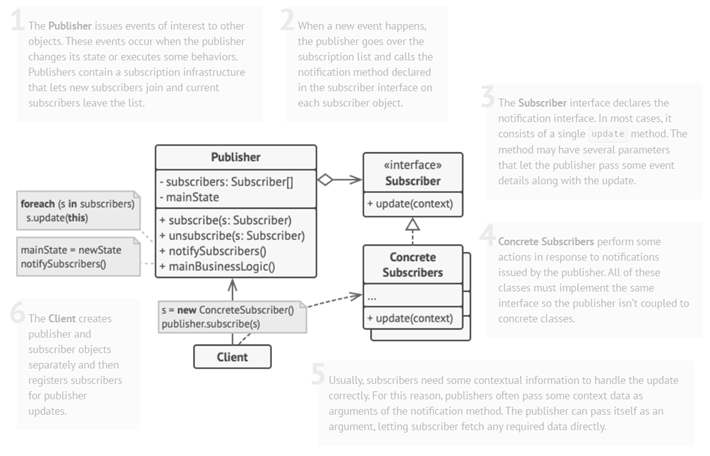
\includegraphics[width=1\textwidth]{../../img/schema_observer.png}
    \caption{Schema del pattern Observer}
    \label{fig:ObserverPattern}
\end{figure}

\end{document}